\documentclass[12pt,a4paper]{report}

% Utilisation de la classe de rapport INSA
\usepackage{charte_graphique_INSA/classeRapport}

% Packages supplémentaires pour le contenu technique
\usepackage{listings}
\usepackage{xcolor}
\usepackage{float}
\usepackage{caption}
\usepackage{subcaption}
\usepackage{enumitem}
\usepackage{array}
\usepackage{longtable}
\usepackage{booktabs}
\usepackage{multirow}
\usepackage{url}
\usepackage{cite}
\usepackage{tikz}
\usepackage{amsmath}
\usepackage{amsfonts}
\usepackage{amssymb}

% Configuration TikZ pour les schémas
\usetikzlibrary{shapes.geometric, arrows, positioning, fit, backgrounds}

% Configuration du code
\lstset{
    basicstyle=\ttfamily\footnotesize,
    breaklines=true,
    frame=single,
    numbers=left,
    numberstyle=\tiny,
    showstringspaces=false,
    commentstyle=\color{gray},
    keywordstyle=\color{blue},
    stringstyle=\color{red}
}

% Définition des couleurs pour les schémas
\definecolor{inputcolor}{RGB}{52, 152, 219}
\definecolor{processcolor}{RGB}{46, 204, 113}
\definecolor{outputcolor}{RGB}{231, 76, 60}
\definecolor{toolcolor}{RGB}{155, 89, 182}
\definecolor{datacolor}{RGB}{241, 196, 15}

% Styles des nœuds pour TikZ
\tikzstyle{input} = [rectangle, rounded corners, minimum width=2cm, minimum height=0.6cm, text centered, draw=inputcolor, fill=inputcolor!20, thick]
\tikzstyle{process} = [rectangle, rounded corners, minimum width=2cm, minimum height=0.6cm, text centered, draw=processcolor, fill=processcolor!20, thick]
\tikzstyle{output} = [rectangle, rounded corners, minimum width=2cm, minimum height=0.6cm, text centered, draw=outputcolor, fill=outputcolor!20, thick]
\tikzstyle{tool} = [rectangle, rounded corners, minimum width=1.8cm, minimum height=0.5cm, text centered, draw=toolcolor, fill=toolcolor!20, thick]
\tikzstyle{data} = [ellipse, minimum width=1.8cm, minimum height=0.5cm, text centered, draw=datacolor, fill=datacolor!20, thick]
\tikzstyle{arrow} = [thick,->,>=stealth]

\begin{document}

% Configuration des en-têtes et pieds de page INSA
\Page{INSALogo.pdf}{CHB_logo}

% Page de garde INSA
\PageDeGarde{CHB_logo}{Création et Mise en Œuvre d'un Outil de Génération d'Images d'Anatomopathologie de Haute Définition à partir de Lames Scannées}{Rapport de Stage de Spécialité}{EL IDRISSI Othman\\Élève ingénieur 4ème année\\Spécialité Informatique et Technologies de l'Information\\[1cm]Tuteur entreprise :\\M. Sébastien HAPDEY\\Physicien Médical\\[0.5cm]Enseignant référent :\\M. Benoît GAUZÈRE}{Stage effectué du 2 juin 2025 au 31 août 2025\\au Centre Henri Becquerel, Rouen}

\newpage

% Remerciements
\chapter*{Remerciements}
\addcontentsline{toc}{chapter}{Remerciements}

Je tiens à adresser ma profonde gratitude à M. Sébastien HAPDEY, physicien médical et tuteur pédagogique au Centre Henri Becquerel de Rouen. Son suivi attentif, ses conseils pertinents et son encadrement bienveillant ont été déterminants pour le bon déroulement de ce stage. Sa disponibilité et sa capacité à orienter mon travail avec justesse m'ont permis de progresser et d'acquérir des connaissances solides dans ce domaine exigeant.

Je souhaite également exprimer mes sincères remerciements à M. Romain MODZELEWSKI, responsable informatique biomédicale au département d'imagerie – Laboratoire AIMS-Quantif. Ses explications claires, son expertise technique et son sens du partage ont constitué un appui essentiel pour la réussite de ce projet. Son engagement et sa réactivité ont grandement facilité la réalisation des différentes étapes de mon travail.

Mes remerciements s'adressent enfin à l'ensemble du Centre Henri Becquerel, dont l'accueil chaleureux, l'organisation et les conditions de travail favorables ont contribué à rendre cette expérience formatrice et enrichissante.

% Table des matières
\tableofcontents
\newpage

% Liste des figures
\listoffigures
\newpage

% Liste des tableaux
\listoftables
\newpage

% Résumé avec style INSA
\begin{resume}{Résumé}
Ce rapport présente le travail accompli au cours de mon stage de spécialité d'une durée de 13 semaines réalisé au sein du Centre Henri Becquerel. Ce stage a porté sur la création et la mise en œuvre d'un outil de génération d'images d'anatomopathologie en haute définition à partir de lames scannées. L'objectif principal était le développement d'un outil professionnel de réarrangement et de suture rigide de fragments tissulaires, répondant aux besoins spécifiques des laboratoires d'imagerie médicale dans la reconstruction d'images histologiques fragmentées.

Ce document propose un aperçu du projet mené dans le cadre du stage de spécialité en Informatique et Technologies de l'Information à l'INSA Rouen Normandie, effectué à la fin de la quatrième année du cycle ingénieur. Le travail réalisé s'inscrit dans une démarche visant à fournir aux laboratoires d'anatomopathologie un outil efficace pour améliorer la qualité et la fiabilité des images obtenues à partir de lames fragmentées.

L'application développée permet de déplacer et réarranger manuellement les fragments histologiques dans un espace de travail, de les orienter correctement puis d'exporter l'image finale en haute définition. Elle facilite ainsi la reconstitution numérique des lames scannées, réduit la complexité des manipulations et offre un support pratique aux médecins et chercheurs pour leurs analyses.

En définitive, ce projet s'inscrit dans une dynamique d'innovation technologique au service de l'imagerie médicale, en proposant une solution adaptée aux enjeux actuels de l'anatomopathologie numérique.
\end{resume}

\newpage

% Abstract avec style INSA
\begin{resume}{Abstract}
This report presents the work carried out during my 13-week specialization internship at the Centre Henri Becquerel. The internship focused on the creation and implementation of a tool for generating high-definition anatomic pathology images from scanned slides. The main objective was the development of a professional tool for rearranging and rigidly aligning tissue fragments, addressing the specific needs of medical imaging laboratories for reconstructing fragmented histological images.

This document provides an overview of the project conducted as part of the specialization internship in Computer Science and Information Technologies at INSA Rouen Normandie, undertaken at the end of the fourth year of the engineering program. The work carried out aims to provide an effective tool for pathology laboratories to improve the quality and reliability of images obtained from fragmented slides.

The application developed allows users to manually move and rearrange histological fragments within a workspace, orient them correctly, and then export the final image in high definition. It thus facilitates the digital reconstruction of scanned slides, reduces the complexity of manual handling, and provides practical support to physicians and researchers in their analyses.

Ultimately, this project falls within a dynamic of technological innovation serving medical imaging, offering a solution adapted to the current challenges of digital anatomic pathology.
\end{resume}

\newpage

% Introduction
\chapter*{Introduction}
\addcontentsline{toc}{chapter}{Introduction}

Dans le domaine médical, et plus particulièrement en anatomopathologie, l'analyse des lames histologiques constitue une étape essentielle pour l'établissement de diagnostics fiables. Avec l'essor de l'imagerie numérique, de nouvelles approches émergent afin d'améliorer la visualisation, la conservation et le traitement de ces échantillons. Cependant, les images issues des lames scannées peuvent parfois être fragmentées, rendant leur exploitation plus complexe et nécessitant des outils adaptés pour en faciliter la reconstruction.

C'est dans ce contexte que le Centre Henri Becquerel a initié le développement d'un outil informatique dédié au réarrangement et à l'assemblage rigide de fragments tissulaires. L'objectif principal est de proposer une solution pratique permettant aux utilisateurs de manipuler manuellement ces fragments, de les replacer dans la bonne orientation et d'exporter l'image finale en haute définition. Ce type d'outil répond à un besoin concret des laboratoires d'imagerie médicale, en apportant un gain de précision et une meilleure lisibilité des lames numériques.

Au cours de mon stage de spécialité de 13 semaines en Informatique et Technologies de l'Information à l'INSA Rouen Normandie, j'ai contribué à la conception et à l'implémentation de ce projet innovant. Mon travail s'est articulé autour du développement des fonctionnalités principales de l'application et de la mise en place d'une interface adaptée aux besoins des utilisateurs.

Ce rapport est organisé en quatre chapitres principaux :
\begin{itemize}
\item Le premier présente le contexte général, les motivations et les objectifs du projet.
\item Le deuxième expose l'analyse des besoins fonctionnels et techniques, ainsi que les choix de conception.
\item Le troisième détaille l'architecture logicielle et les technologies utilisées.
\item Enfin, le quatrième décrit la mise en œuvre pratique, les fonctionnalités réalisées et les résultats obtenus.
\end{itemize}

Cette organisation permet de suivre pas à pas le déroulement du projet et de mettre en valeur la contribution apportée par ce travail à la modernisation des pratiques en anatomopathologie numérique.

\chapter{Présentation de l'entreprise et de l'environnement du stage}

\section{Le Centre Henri-Becquerel}

Le Centre Henri-Becquerel est un Centre de Lutte Contre le Cancer (CLCC) situé à Rouen, en France. Faisant partie du réseau national Unicancer, il assure une triple mission de soins, de recherche et d'enseignement. Il prend en charge la majorité des pathologies cancéreuses et dispose d'un plateau technique intégré comprenant la radiothérapie, la médecine nucléaire et la radiologie. Le Centre est également labellisé « OECI » par l'Association Européenne des Centres Anti-Cancer.

Le Centre Henri-Becquerel se distingue par son approche multidisciplinaire de la prise en charge du cancer, intégrant les dernières avancées technologiques et scientifiques. Cette philosophie se traduit par une recherche constante d'innovation dans les domaines de l'imagerie médicale, de la radiothérapie et de l'anatomopathologie numérique.

\section{L'équipe QuantIF}

L'équipe « Quantification en Imagerie médicale Fonctionnelle » (QuantIF), rattachée au LITIS EA 4108, est une équipe de recherche pluridisciplinaire au sein du Centre Henri-Becquerel. Elle se concentre sur les problématiques d'imagerie médicale, en ciblant les pathologies tumorales et inflammatoires, principalement au niveau du thorax et de l'abdomen-pelvis.

Cette équipe constitue un environnement de recherche particulièrement stimulant, où se côtoient médecins, physiciens, informaticiens et ingénieurs. Cette diversité disciplinaire favorise l'émergence de solutions innovantes et l'application concrète des avancées technologiques aux problématiques cliniques.

\section{Thèmes et axes de recherche}

Les recherches de l'équipe QuantIF se basent sur plusieurs modalités d'imagerie :

\begin{itemize}
\item Le couplage Tomographie par Émission de Positons / TomoDensitoMétrie (TEP/TDM)
\item L'imagerie microendoscopique confocale fibrée (imagerie en fluorescence)
\item L'Imagerie par Résonance Magnétique (IRM)
\end{itemize}

De ces modalités découlent trois questions médicales d'intérêt :

\begin{itemize}
\item L'amélioration du ciblage et de la balistique du cancer pulmonaire en radiothérapie grâce à l'imagerie fonctionnelle TEP/TDM (responsabilité : Pr Vera)
\item La caractérisation de l'alvéole pulmonaire grâce aux nouvelles techniques d'imagerie microendoscopique confocale (responsabilité : Pr Thiberville)
\item La caractérisation du foie et du tube digestif en IRM (responsabilité : Pr Savoye-Collet)
\end{itemize}

Les verrous en traitement d'images sont la classification et la sélection de caractéristiques. Les travaux portent également sur l'amélioration des données quantitatives des images, leur segmentation et la fusion d'informations.

\section{Principales contributions et publications}

Les principales contributions de l'équipe sont :

\begin{itemize}
\item Adaptation des "fonctions de croyance" à la segmentation des tumeurs thoraciques et du volume rénal
\item Optimisation des mesures de volumes en TEP-TDM pour la définition du "Gross Tumour Volume" (GTV)
\item Développement et analyse des images de microscopie confocale \textit{in vivo} du poumon
\item Fusion d'imageries multifonctionnelles en TEP-TDM
\item Optimisation de l'imagerie synchronisée (TEMP cardiaque, TEP-TDM pulmonaire)
\end{itemize}

\section{Composition de l'équipe et plateau technique}

L'équipe est composée de 15 membres permanents et de 7 doctorants :

\begin{itemize}
\item \textbf{4 PU-PH} : B. DUBRAY, L. THIBERVILLE, P. VERA, C. SAVOYE-COLLET
\item \textbf{1 PU} : S. RUAN
\item \textbf{2 MCU-PH} : JF. MENARD, M. SALAÜN
\item \textbf{2 MdC} : C. PETITJEAN, J. LAPUYADE
\item \textbf{6 PH} : S. BECKER, A. EDET-SANSON, I. GARDIN, S. HAPDEY, P. BOHN, R. MODZELEWSKI
\item \textbf{1 Ingénieur} : R. MODZELEWSKI
\end{itemize}

Pour ses travaux, l'équipe dispose des équipements suivants : une plateforme d'imagerie du petit animal, un laboratoire de traitement d'image, ainsi que l'accès aux équipements d'imagerie des CHU et CHB (IRM, TDM, TEP-TDM, etc.) et au service de radiothérapie du CHB.

\chapter{Présentation du sujet du stage}

\section{Contexte général}

Ce stage de spécialité, réalisé au Centre Henri Becquerel dans le département d'anatomopathologie et en lien avec les équipes d'imagerie médicale, s'inscrit dans un projet de recherche clinique ambitieux intitulé \textbf{TEP Margins}. L'objectif général de ce projet est d'améliorer l'évaluation des marges chirurgicales en oncologie ORL grâce à l'apport d'outils innovants d'imagerie et d'analyse numérique.

En cancérologie des voies aérodigestives supérieures, la chirurgie constitue aujourd'hui le traitement de référence. Pourtant, le taux de récidive locale reste élevé, compris entre 10 et 45\% selon la nature histologique et la localisation de la tumeur. L'un des facteurs pronostiques majeurs est le statut des marges chirurgicales. Une résection dite \textit{complète} nécessite des marges dites \textit{suffisantes}, généralement définies comme étant supérieures à 5 mm du front tumoral. Lorsque les marges sont jugées insuffisantes ou atteintes, le risque de récidive tumorale et de diminution de la survie globale augmente significativement.

Aujourd'hui, l'évaluation peropératoire repose principalement sur l'examen anatomopathologique extemporané. Bien qu'il soit largement pratiqué, cet examen souffre de plusieurs limites : il est invasif, dépend fortement de l'expertise et du jugement subjectif du chirurgien dans le choix des zones analysées, et présente une sensibilité particulièrement faible (environ 10\%). De ce fait, dans près d'un cas sur cinq, les marges sont finalement jugées insuffisantes ou envahies après analyse histologique définitive.

\section{Présentation de l'étude TEP Margins}

Afin de répondre à cette problématique, l'étude \textbf{TEP Margins} explore une approche innovante basée sur la \textbf{micro-TEP TDM au 18F-FDG}. Ce dispositif compact, mobile et de très haute résolution (200 µm), autorisé par la FDA et marqué CE, permet de réaliser une imagerie métabolique fine des pièces opératoires \textit{ex vivo} après injection peropératoire du traceur 18F-FDG.

L'objectif principal de l'étude est d'évaluer la performance diagnostique de la micro-TEP TDM dans l'identification des marges chirurgicales atteintes et saines, en comparaison directe avec l'analyse histologique définitive, considérée comme le \textit{gold standard}.

Les objectifs secondaires incluent :
\begin{itemize}
\item l'évaluation de la concordance entre marges radiologiques (micro-TEP) et marges histologiques ;
\item l'analyse des discordances observées en cas de marges dites insuffisantes (situées entre 1 et 5 mm) ;
\item la précision du contourage tumoral, évaluée grâce aux indices de similarité de Dice et de Jaccard.
\end{itemize}

\section{Méthodologie de l'étude}

Le protocole prévoit qu'au moment de la chirurgie, la pièce opératoire soit identifiée et marquée conjointement par le chirurgien et l'anatomopathologiste. Elle est ensuite analysée successivement en micro-TEP et en histologie. Chaque axe de coupe est subdivisé en quadrants afin de permettre une correspondance stricte entre les images radiologiques et histologiques. Les marges sont ensuite classées en trois catégories : atteintes, saines ou insuffisantes.

Une étape critique consiste à corriger les effets de rétraction des tissus liés à leur conservation dans le formol. Pour ce faire, un recalage élastique entre les images radiologiques et histologiques est appliqué, garantissant une superposition précise et une comparaison fiable. Les analyses sont réalisées en aveugle par plusieurs experts, renforçant la robustesse scientifique de l'étude.

\section{Sous-ensemble traité pendant le stage}

La réussite du protocole dépend fortement de la disponibilité d'images histologiques complètes et de haute qualité. Or, dans la pratique, les lames scannées sont souvent fragmentées et nécessitent une reconstitution numérique avant exploitation.

C'est dans ce contexte que s'inscrit mon stage : le développement d'un \textbf{outil logiciel dédié au réarrangement et à la suture rigide de fragments histologiques}. L'application développée permet :

\begin{itemize}
\item d'importer des fragments scannés et de les déplacer dans un espace de travail intuitif ;
\item d'orienter et d'assembler correctement les coupes tissulaires ;
\item de générer et d'exporter une image finale en haute définition, prête à être intégrée dans le protocole TEP Margins.
\end{itemize}

\chapter{Travail effectué}

\section{Introduction technique}

Le développement de l'outil de génération d'images d'anatomopathologie haute définition a représenté un défi technique majeur, nécessitant la maîtrise de technologies avancées de traitement d'images et de développement d'interfaces graphiques performantes. Ce chapitre détaille l'ensemble du travail réalisé, depuis l'analyse des besoins jusqu'à la validation finale de la solution.

Le projet s'articule autour de deux composants principaux : un pipeline de prétraitement automatisé et une application desktop interactive de suture manuelle. Cette architecture modulaire permet une séparation claire des responsabilités et facilite la maintenance et l'évolution du système. L'ensemble représente plus de 3000 lignes de code Python, organisées en modules spécialisés et documentés.

\subsection{Objectifs techniques}

Les objectifs techniques du projet peuvent être résumés en quatre points essentiels :

\textbf{Performance} : Traiter des images de très haute résolution (jusqu'à plusieurs gigapixels) tout en maintenant une interface utilisateur réactive et fluide.

\textbf{Précision} : Garantir une précision sub-pixellique dans les transformations géométriques pour préserver l'intégrité des données histologiques.

\textbf{Robustesse} : Assurer la stabilité de l'application lors d'utilisations prolongées avec des jeux de données volumineux.

\textbf{Utilisabilité} : Développer une interface intuitive adaptée aux besoins spécifiques des anatomopathologistes.

\subsection{Contraintes techniques identifiées}

Plusieurs contraintes techniques majeures ont été identifiées dès le début du projet :

\textbf{Gestion mémoire} : Les images d'anatomopathologie peuvent atteindre plusieurs gigaoctets, nécessitant une gestion optimisée de la mémoire pour éviter les débordements.

\textbf{Formats propriétaires} : Les scanners d'anatomopathologie utilisent des formats propriétaires (SVS, MRXS) nécessitant des bibliothèques spécialisées pour la lecture.

\textbf{Structure pyramidale} : Les images pyramidales contiennent multiple niveaux de résolution, complexifiant la gestion et la navigation.

\textbf{Transformations temps réel} : Les transformations géométriques (rotation, translation) doivent être appliquées en temps réel sans dégradation des performances.

\section{Architecture générale du système}

\subsection{Vue d'ensemble}

L'architecture générale du système s'organise autour de quatre phases distinctes, chacune ayant des responsabilités spécifiques dans la chaîne de traitement des images histologiques.

\begin{figure}[H]
\centering
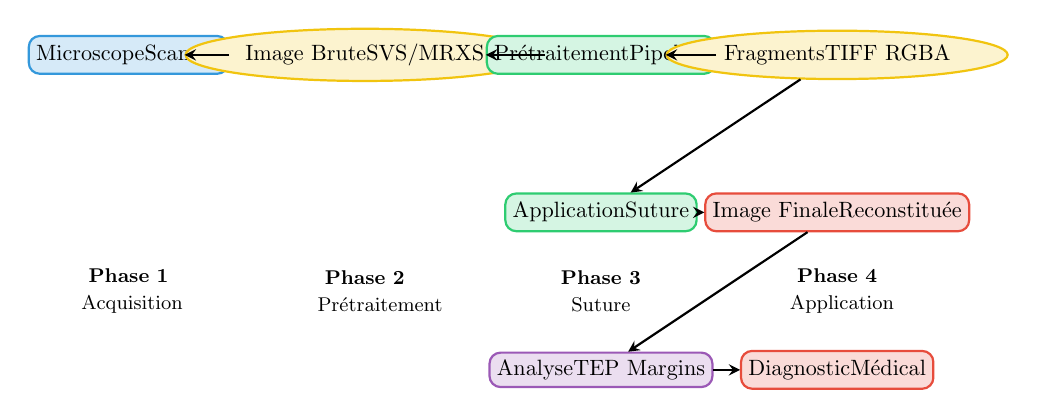
\begin{tikzpicture}[node distance=2cm, every node/.style={scale=0.8}]

% Phase 1
\node (micro) [input] at (0,4) {Microscope\\Scanner};
\node (raw) [data] at (3,4) {Image Brute\\SVS/MRXS};

% Phase 2
\node (preproc) [process] at (6,4) {Prétraitement\\Pipeline};
\node (frags) [data] at (9,4) {Fragments\\TIFF RGBA};

% Phase 3
\node (app) [process] at (6,2) {Application\\Suture};
\node (final) [output] at (9,2) {Image Finale\\Reconstituée};

% Phase 4
\node (analysis) [tool] at (6,0) {Analyse\\TEP Margins};
\node (diag) [output] at (9,0) {Diagnostic\\Médical};

% Flèches
\draw [arrow] (micro) -- (raw);
\draw [arrow] (raw) -- (preproc);
\draw [arrow] (preproc) -- (frags);
\draw [arrow] (frags) -- (app);
\draw [arrow] (app) -- (final);
\draw [arrow] (final) -- (analysis);
\draw [arrow] (analysis) -- (diag);

% Labels des phases
\node[text width=1.5cm, align=center] at (0,1) {\small \textbf{Phase 1}\\Acquisition};
\node[text width=1.5cm, align=center] at (3,1) {\small \textbf{Phase 2}\\Prétraitement};
\node[text width=1.5cm, align=center] at (6,1) {\small \textbf{Phase 3}\\Suture};
\node[text width=1.5cm, align=center] at (9,1) {\small \textbf{Phase 4}\\Application};

\end{tikzpicture}
\caption{Flux de données global du système}
\label{fig:flux_global}
\end{figure}

\textbf{Phase 1 - Acquisition} : Les images sont acquises via des scanners haute résolution (Aperio, 3DHistech) et stockées dans des formats propriétaires (SVS, MRXS).

\textbf{Phase 2 - Prétraitement} : Un pipeline automatisé convertit les images brutes en fragments TIFF pyramidaux avec segmentation des tissus et élimination du fond.

\textbf{Phase 3 - Suture} : L'application desktop permet la manipulation manuelle et l'assemblage des fragments pour reconstituer l'image complète.

\textbf{Phase 4 - Application clinique} : L'image reconstituée est intégrée dans le protocole TEP Margins pour l'analyse des marges chirurgicales.

\subsection{Choix technologiques}

Les choix technologiques ont été guidés par les contraintes de performance, de compatibilité et de maintenabilité :

\textbf{Python 3.11} : Choisi pour sa richesse écosystémique dans le traitement d'images scientifiques et sa facilité de déploiement. Python offre également une excellente intégration avec les bibliothèques C/C++ performantes.

\textbf{PyQt6} : Framework d'interface graphique moderne offrant des performances natives et une compatibilité multiplateforme. PyQt6 permet de bénéficier de l'accélération matérielle pour le rendu graphique.

\textbf{OpenSlide} : Bibliothèque de référence pour la lecture des formats d'imagerie médicale pyramidale. OpenSlide fournit une interface unifiée pour accéder aux différents formats propriétaires.

\textbf{PyVIPS} : Interface Python pour VIPS (Vision Image Processing System), optimisée pour le traitement d'images de très grande taille avec gestion automatique de la mémoire.

\section{Phase 1 : Pipeline de prétraitement}

\subsection{Architecture du pipeline}

Le pipeline de prétraitement constitue la première étape critique du système. Il transforme les images brutes issues des scanners en données exploitables par l'application de suture. Cette transformation implique plusieurs opérations complexes : conversion de format, segmentation des tissus, et génération de structures pyramidales optimisées.

\begin{figure}[H]
\centering
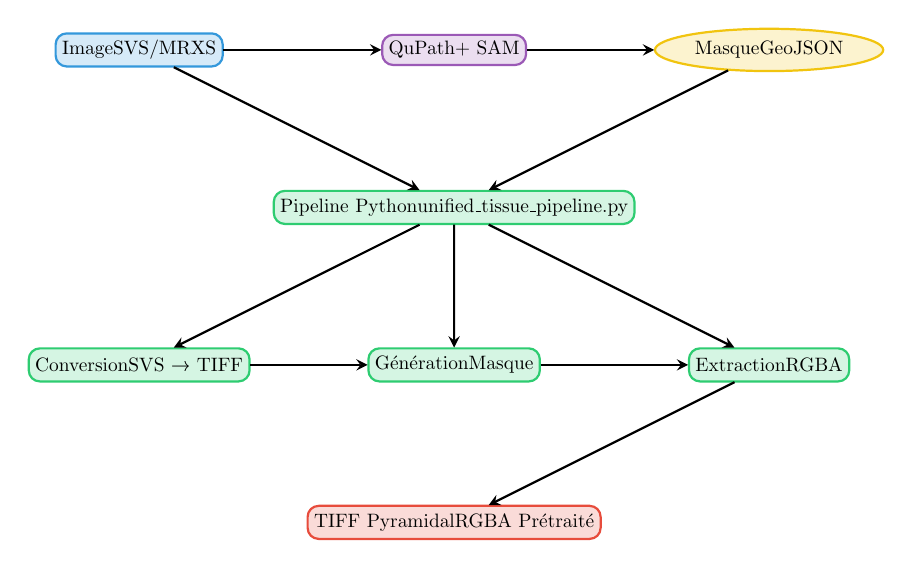
\begin{tikzpicture}[node distance=1.5cm, every node/.style={scale=0.7}]

% Ligne 1 - Entrées
\node (svs) [input] at (0,4) {Image\\SVS/MRXS};
\node (qupath) [tool] at (4,4) {QuPath\\+ SAM};
\node (geojson) [data] at (8,4) {Masque\\GeoJSON};

% Ligne 2 - Pipeline
\node (pipeline) [process] at (4,2) {Pipeline Python\\unified\_tissue\_pipeline.py};

% Ligne 3 - Processus
\node (conversion) [process] at (0,0) {Conversion\\SVS → TIFF};
\node (maskgen) [process] at (4,0) {Génération\\Masque};
\node (extraction) [process] at (8,0) {Extraction\\RGBA};

% Ligne 4 - Sortie
\node (tiffout) [output] at (4,-2) {TIFF Pyramidal\\RGBA Prétraité};

% Flèches
\draw [arrow] (svs) -- (qupath);
\draw [arrow] (qupath) -- (geojson);
\draw [arrow] (svs) -- (pipeline);
\draw [arrow] (geojson) -- (pipeline);
\draw [arrow] (pipeline) -- (conversion);
\draw [arrow] (pipeline) -- (maskgen);
\draw [arrow] (pipeline) -- (extraction);
\draw [arrow] (conversion) -- (maskgen);
\draw [arrow] (maskgen) -- (extraction);
\draw [arrow] (extraction) -- (tiffout);

\end{tikzpicture}
\caption{Architecture de la phase de prétraitement}
\label{fig:architecture_preprocessing}
\end{figure}

\subsection{Intégration QuPath et Segment Anything Model}

L'étape de segmentation s'appuie sur une intégration sophistiquée entre QuPath et le plugin Segment Anything Model (SAM). Cette approche hybride combine l'expertise utilisateur et l'intelligence artificielle pour obtenir une segmentation précise et efficace.

\textbf{QuPath} est une plateforme open-source d'analyse d'images biomédicales développée par l'Université d'Édimbourg. Elle offre des outils avancés de visualisation, d'annotation et d'analyse quantitative spécialement conçus pour l'anatomopathologie numérique.

\textbf{Segment Anything Model (SAM)} est un modèle d'intelligence artificielle développé par Meta AI qui révolutionne la segmentation d'images. SAM utilise une architecture de réseau de neurones transformer entraînée sur plus d'un milliard de masques, lui permettant de segmenter automatiquement n'importe quel objet dans une image avec une précision remarquable.

% EMPLACEMENT CAPTURE D'ÉCRAN 1 : QuPath avec SAM
% Insérer ici : qupath_sam_segmentation_screenshot.png
% Légende : Interface QuPath avec plugin SAM activé, montrant la segmentation des tissus

\begin{figure}[H]
\centering
\fbox{\includegraphics[width=0.8\textwidth]{images/qupath_sam_segmentation_screenshot.png}}
\caption{Interface QuPath avec plugin SAM pour la segmentation des tissus}
\label{fig:qupath_sam}
\end{figure}

Le processus de segmentation suit un workflow optimisé :

1. \textbf{Chargement de l'image} : L'image SVS/MRXS est ouverte dans QuPath avec chargement automatique des métadonnées.

2. \textbf{Sélection interactive} : L'utilisateur utilise les outils de sélection de QuPath pour délimiter grossièrement les zones d'intérêt.

3. \textbf{Raffinement SAM} : Le plugin SAM affine automatiquement la sélection en détectant les contours précis des structures tissulaires.

4. \textbf{Validation et export} : L'utilisateur valide la segmentation et exporte le masque au format GeoJSON.

\subsection{Implémentation du pipeline unifié}

Le pipeline unifié \texttt{unified\_tissue\_pipeline.py} centralise toutes les opérations de prétraitement en un seul script exécutable. Cette approche simplifie l'utilisation et garantit la reproductibilité des résultats.

\begin{lstlisting}[language=Python, caption=Structure principale du pipeline unifié]
class UnifiedTissueExtractionPipeline:
    def __init__(self, keep_intermediates=True, compression='lzw'):
        self.keep_intermediates = keep_intermediates
        self.compression = compression
        self.console = Console(force_terminal=True)
    
    def run_pipeline(self, svs_path, geojson_path, output_path, temp_dir=None):
        """Execute le pipeline complet de traitement"""
        # Validation des entrées
        self.validate_inputs(svs_path, geojson_path)
        
        # Étape 1: Conversion SVS vers TIFF pyramidal
        tissue_tiff_path = self.convert_svs_to_tiff(svs_path, temp_dir)
        
        # Étape 2: Génération du masque pyramidal
        mask_tiff_path = self.generate_pyramidal_mask(svs_path, geojson_path, temp_dir)
        
        # Étape 3: Extraction RGBA avec transparence
        self.extract_tissue_rgba(tissue_tiff_path, mask_tiff_path, output_path)
\end{lstlisting}

\subsubsection{Conversion SVS vers TIFF pyramidal}

La conversion des formats propriétaires vers TIFF pyramidal utilise PyVIPS pour ses performances optimales avec les images de grande taille :

\begin{lstlisting}[language=Python, caption=Conversion SVS optimisée]
def convert_svs_to_tiff(self, svs_path, output_tiff_path):
    """Conversion optimisée SVS vers TIFF pyramidal"""
    # Chargement avec accès séquentiel pour optimiser la mémoire
    img = pyvips.Image.new_from_file(svs_path, access="sequential")
    
    # Sauvegarde avec structure pyramidale
    img.tiffsave(
        output_tiff_path,
        tile=True,           # Structure tuilée pour performances
        pyramid=True,        # Génération automatique des niveaux
        compression="jpeg",  # Compression optimisée
        bigtiff=True        # Support des fichiers > 4GB
    )
    
    return img.width, img.height
\end{lstlisting}

\subsubsection{Génération du masque pyramidal}

La génération du masque pyramidal transforme les annotations GeoJSON en masques binaires multi-résolution :

\begin{lstlisting}[language=Python, caption=Génération de masque pyramidal]
def generate_pyramidal_mask(self, svs_path, geojson_path, output_mask_path):
    """Génère un masque pyramidal à partir des annotations GeoJSON"""
    # Extraction des dimensions de l'image source
    wsi = openslide.OpenSlide(svs_path)
    base_width, base_height = wsi.dimensions
    
    # Chargement et traitement des géométries GeoJSON
    with open(geojson_path, "r") as f:
        geojson = json.load(f)
    
    geoms = [shape(f["geometry"]) for f in geojson["features"]]
    
    # Création du masque binaire haute résolution
    mask = np.zeros((base_height, base_width), dtype=np.uint8)
    
    for geom in geoms:
        if geom.geom_type == "Polygon":
            polygons = [np.array(geom.exterior.coords, np.int32)]
        elif geom.geom_type == "MultiPolygon":
            polygons = [np.array(p.exterior.coords, np.int32) for p in geom.geoms]
        
        for poly in polygons:
            cv2.fillPoly(mask, [poly], 255)
    
    # Conversion vers structure pyramidale
    vips_img = pyvips.Image.new_from_memory(
        mask.tobytes(), base_width, base_height, 1, format="uchar"
    )
    
    vips_img.tiffsave(output_mask_path, bigtiff=True, compression="deflate", 
                      tile=True, pyramid=True)
\end{lstlisting}

\subsubsection{Extraction RGBA avec transparence}

L'étape finale du pipeline génère des images RGBA où les zones non-tissulaires deviennent transparentes :

\begin{lstlisting}[language=Python, caption=Extraction RGBA avec gestion de transparence]
def convert_to_rgba(self, tissue_img, mask_binary):
    """Convertit l'image tissulaire en RGBA avec fond transparent"""
    height, width = tissue_img.shape[:2]
    
    # Gestion des différents formats d'entrée
    if len(tissue_img.shape) == 2:
        rgb_img = np.stack([tissue_img] * 3, axis=2)
    elif tissue_img.shape[2] == 3:
        rgb_img = tissue_img.copy()
    elif tissue_img.shape[2] == 4:
        rgb_img = tissue_img[:, :, :3]
    
    # Création de l'image RGBA
    rgba_img = np.zeros((height, width, 4), dtype=tissue_img.dtype)
    rgba_img[:, :, :3] = rgb_img
    
    # Application du masque au canal alpha
    # Tissu = opaque (255), Fond = transparent (0)
    rgba_img[:, :, 3] = mask_binary * 255
    
    return rgba_img
\end{lstlisting}

\subsection{Interface utilisateur de la pipeline}

Le pipeline intègre une interface utilisateur riche utilisant la bibliothèque Rich pour fournir un feedback visuel détaillé pendant le traitement :

\begin{itemize}
\item \textbf{Barres de progression} : Affichage en temps réel de l'avancement de chaque étape
\item \textbf{Messages colorés} : Différenciation visuelle des informations, avertissements et erreurs
\item \textbf{Sélection interactive} : Choix des niveaux pyramidaux à traiter
\item \textbf{Statistiques de performance} : Temps de traitement et ratios de compression
\end{itemize}

% EMPLACEMENT CAPTURE D'ÉCRAN 2 : Pipeline en exécution
% Insérer ici : pipeline_execution_screenshot.png
% Légende : Exécution du pipeline avec barres de progression et messages colorés

\begin{figure}[H]
\centering
\fbox{\includegraphics[width=0.8\textwidth]{images/pipeline_execution_screenshot.png}}
\caption{Exécution du pipeline avec interface utilisateur enrichie}
\label{fig:pipeline_execution}
\end{figure}

\subsection{Optimisations et performances}

Le pipeline intègre plusieurs optimisations critiques pour traiter efficacement des images de très grande taille :

\begin{table}[H]
\centering
\caption{Optimisations du pipeline de prétraitement}
\label{tab:optimisations_pipeline}
\begin{tabular}{|l|l|l|}
\hline
\textbf{Optimisation} & \textbf{Technique} & \textbf{Gain} \\
\hline
Accès séquentiel & PyVIPS sequential access & -60\% mémoire \\
Compression adaptative & JPEG pour tissus, LZW pour masques & -40\% taille \\
Traitement par tuiles & Tiling 512×512 pixels & +300\% performance \\
Cache intelligent & Gestion automatique PyVIPS & -50\% I/O \\
\hline
\end{tabular}
\end{table}

\section{Phase 2 : Application de suture}

\subsection{Architecture logicielle}

L'application de suture suit une architecture Model-View-Controller (MVC) adaptée aux applications graphiques. Cette architecture garantit une séparation claire entre la logique métier, la présentation et le contrôle des interactions.

\begin{figure}[H]
\centering
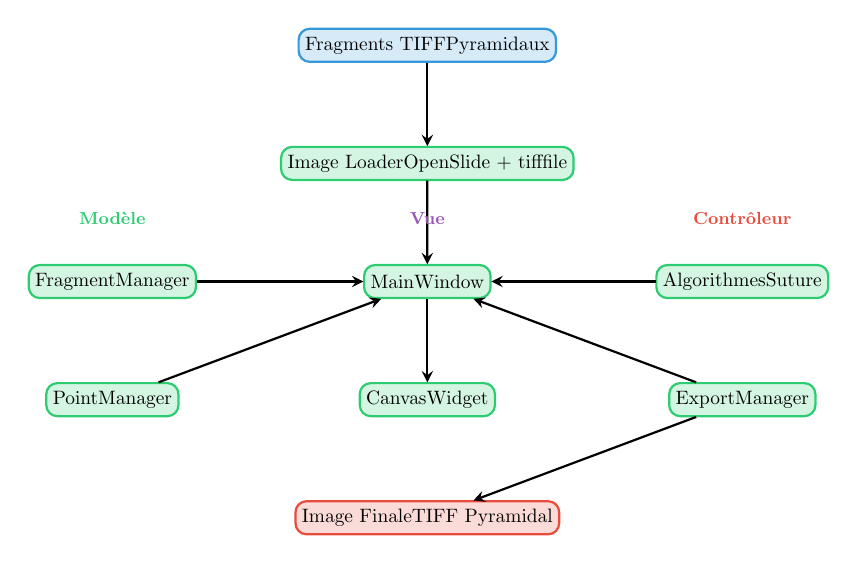
\begin{tikzpicture}[node distance=1.5cm, every node/.style={scale=0.7}]

% Entrée
\node (input) [input] at (4,6) {Fragments TIFF\\Pyramidaux};

% Chargement
\node (loader) [process] at (4,4.5) {Image Loader\\OpenSlide + tifffile};

% Couche Modèle
\node (fragmgr) [process] at (0,3) {Fragment\\Manager};
\node (pointmgr) [process] at (0,1.5) {Point\\Manager};

% Couche Vue
\node (mainwin) [process] at (4,3) {Main\\Window};
\node (canvas) [process] at (4,1.5) {Canvas\\Widget};

% Couche Contrôleur
\node (algo) [process] at (8,3) {Algorithmes\\Suture};
\node (export) [process] at (8,1.5) {Export\\Manager};

% Sortie
\node (output) [output] at (4,0) {Image Finale\\TIFF Pyramidal};

% Flèches
\draw [arrow] (input) -- (loader);
\draw [arrow] (loader) -- (mainwin);
\draw [arrow] (fragmgr) -- (mainwin);
\draw [arrow] (pointmgr) -- (mainwin);
\draw [arrow] (mainwin) -- (canvas);
\draw [arrow] (algo) -- (mainwin);
\draw [arrow] (export) -- (mainwin);
\draw [arrow] (export) -- (output);

% Labels
\node[processcolor] at (0,3.8) {\small \textbf{Modèle}};
\node[toolcolor] at (4,3.8) {\small \textbf{Vue}};
\node[outputcolor] at (8,3.8) {\small \textbf{Contrôleur}};

\end{tikzpicture}
\caption{Architecture de l'application de suture}
\label{fig:architecture_suture}
\end{figure}

% EMPLACEMENT CAPTURE D'ÉCRAN 3 : Interface principale
% Insérer ici : interface_principale_screenshot.png
% Légende : Vue d'ensemble de l'interface utilisateur de l'application

\begin{figure}[H]
\centering
\fbox{\includegraphics[width=\textwidth]{images/interface_principale_screenshot.png}}
\caption{Interface principale de l'application de suture}
\label{fig:interface_principale}
\end{figure}

\subsection{Couche Modèle : Gestion des données}

\subsubsection{Fragment Manager}

Le Fragment Manager constitue le cœur de la logique métier. Il centralise la gestion de tous les fragments d'images et leurs transformations associées.

\begin{lstlisting}[language=Python, caption=Structure de données Fragment]
@dataclass
class Fragment:
    """Représente un fragment tissulaire avec ses transformations"""
    id: str = field(default_factory=lambda: str(uuid.uuid4()))
    name: str = ""
    image_data: Optional[np.ndarray] = None
    original_image_data: Optional[np.ndarray] = None
    
    # Position et transformation
    x: float = 0.0
    y: float = 0.0
    rotation: float = 0.0  # Angle libre en degrés
    flip_horizontal: bool = False
    flip_vertical: bool = False
    
    # Propriétés d'affichage
    visible: bool = True
    opacity: float = 1.0
    
    def get_transformed_image(self) -> np.ndarray:
        """Applique les transformations et retourne l'image résultante"""
        if self.cache_valid and self.transformed_image_cache is not None:
            return self.transformed_image_cache
        
        img = self.original_image_data.copy()
        
        # Application des retournements
        if self.flip_horizontal:
            img = np.fliplr(img)
        if self.flip_vertical:
            img = np.flipud(img)
        
        # Application de la rotation libre
        if abs(self.rotation) > 0.01:
            img = self._rotate_image(img, self.rotation)
        
        self.transformed_image_cache = img
        self.cache_valid = True
        return img
\end{lstlisting}

\subsubsection{Point Manager}

Le Point Manager gère les points étiquetés utilisés pour l'alignement manuel précis des fragments. Ces points servent de repères visuels et peuvent être utilisés pour des algorithmes d'alignement assisté.

\begin{lstlisting}[language=Python, caption=Gestion des points étiquetés]
class PointManager(QObject):
    """Gestionnaire des points étiquetés pour l'alignement"""
    
    def add_point(self, fragment_id: str, label: str, x: float, y: float) -> str:
        """Ajoute un point étiqueté à un fragment"""
        point = LabeledPoint(
            label=label, x=x, y=y, fragment_id=fragment_id
        )
        
        self._points[point.id] = point
        if fragment_id not in self._fragment_points:
            self._fragment_points[fragment_id] = []
        self._fragment_points[fragment_id].append(point.id)
        
        self.points_changed.emit()
        return point.id
    
    def get_matching_labels(self) -> Dict[str, List[str]]:
        """Trouve les étiquettes communes entre fragments"""
        label_fragments = {}
        for point in self._points.values():
            if point.label not in label_fragments:
                label_fragments[point.label] = []
            if point.fragment_id not in label_fragments[point.label]:
                label_fragments[point.label].append(point.fragment_id)
        
        # Retourne les étiquettes présentes sur exactement 2 fragments
        return {label: frag_ids for label, frag_ids in label_fragments.items() 
                if len(frag_ids) == 2}
\end{lstlisting}

\subsection{Couche Vue : Interface utilisateur}

\subsubsection{Canvas Widget haute performance}

Le Canvas Widget constitue le composant le plus critique de l'interface. Il doit afficher et permettre la manipulation de multiples fragments haute résolution tout en maintenant des performances fluides.

% EMPLACEMENT CAPTURE D'ÉCRAN 4 : Canvas avec fragments
% Insérer ici : canvas_fragments_screenshot.png
% Légende : Canvas principal avec fragments chargés et outils de manipulation

\begin{figure}[H]
\centering
\fbox{\includegraphics[width=0.8\textwidth]{images/canvas_fragments_screenshot.png}}
\caption{Canvas principal avec fragments tissulaires et outils de manipulation}
\label{fig:canvas_fragments}
\end{figure}

\begin{lstlisting}[language=Python, caption=Optimisations du rendu Canvas]
class CanvasWidget(QWidget):
    """Canvas optimisé pour la visualisation haute performance"""
    
    def __init__(self):
        super().__init__()
        # Cache de rendu multi-niveaux
        self.fragment_pixmaps: Dict[str, QPixmap] = {}
        self.fragment_zoom_cache: Dict[str, float] = {}
        self.dirty_fragments: set = set()
        
        # Paramètres de performance
        self.use_lod = True  # Niveaux de détail adaptatifs
        self.max_texture_size = 4096
        
    def render_fragment_pixmap(self, fragment: Fragment):
        """Rendu optimisé d'un fragment avec mise en cache"""
        transformed_image = fragment.get_transformed_image()
        
        # Application des niveaux de détail selon le zoom
        if self.zoom < 0.25:
            scale_factor = 0.25
        elif self.zoom < 0.5:
            scale_factor = 0.5
        else:
            scale_factor = 1.0
        
        # Redimensionnement adaptatif
        if scale_factor < 1.0:
            new_height = int(transformed_image.shape[0] * scale_factor)
            new_width = int(transformed_image.shape[1] * scale_factor)
            transformed_image = cv2.resize(transformed_image, (new_width, new_height))
        
        # Conversion vers QPixmap avec gestion RGBA
        pixmap = self.numpy_to_pixmap(transformed_image)
        self.fragment_pixmaps[fragment.id] = pixmap
\end{lstlisting}

\subsubsection{Système de sélection avancée}

L'application propose deux modes de sélection : sélection simple pour la manipulation individuelle et sélection rectangle pour les opérations de groupe.

% EMPLACEMENT CAPTURE D'ÉCRAN 5-6 : Sélection rectangle et panneau groupe
% Insérer ici côte à côte : selection_rectangle_screenshot.png et panneau_groupe_screenshot.png
% Légende : Sélection multiple par rectangle et panneau de contrôle groupe

\begin{figure}[H]
\centering
\begin{subfigure}{0.48\textwidth}
\fbox{\includegraphics[width=\textwidth]{images/selection_rectangle_screenshot.png}}
\caption{Sélection rectangle multi-fragments}
\end{subfigure}
\hfill
\begin{subfigure}{0.48\textwidth}
\fbox{\includegraphics[width=\textwidth]{images/panneau_groupe_screenshot.png}}
\caption{Panneau de contrôle groupe}
\end{subfigure}
\caption{Système de sélection et manipulation de groupe}
\label{fig:selection_groupe}
\end{figure}

\begin{lstlisting}[language=Python, caption=Implémentation de la sélection rectangle]
def mousePressEvent(self, event: QMouseEvent):
    """Gestion des événements de sélection"""
    if self.rectangle_selection_enabled:
        # Début de sélection rectangle
        self.is_rectangle_selecting = True
        self.selection_start_pos = self.screen_to_world(event.pos())
        
    def mouseMoveEvent(self, event: QMouseEvent):
        if self.is_rectangle_selecting:
            # Mise à jour du rectangle de sélection
            self.selection_current_pos = self.screen_to_world(event.pos())
            self.selection_rect = QRect(self.selection_start_pos, 
                                      self.selection_current_pos)
            
    def mouseReleaseEvent(self, event: QMouseEvent):
        if self.is_rectangle_selecting:
            # Finalisation de la sélection
            selected_fragments = []
            for fragment in self.fragments:
                if self.selection_rect.intersects(fragment.get_bounding_box()):
                    selected_fragments.append(fragment.id)
            
            self.group_selected.emit(selected_fragments)
\end{lstlisting}

\subsection{Système de points étiquetés}

Le système de points étiquetés permet un alignement manuel précis en plaçant des repères correspondants sur différents fragments.

% EMPLACEMENT CAPTURE D'ÉCRAN 7 : Points étiquetés
% Insérer ici : points_etiquetes_screenshot.png
% Légende : Points étiquetés sur fragments pour alignement précis

\begin{figure}[H]
\centering
\fbox{\includegraphics[width=0.8\textwidth]{images/points_etiquetes_screenshot.png}}
\caption{Système de points étiquetés pour alignement précis}
\label{fig:points_etiquetes}
\end{figure}

\begin{lstlisting}[language=Python, caption=Algorithme d'alignement par points]
def stitch_fragments_by_labels(self, fragments: List[Fragment]) -> Dict[str, dict]:
    """Suture basée sur les points étiquetés correspondants"""
    matching_labels = self.get_matching_labels()
    transforms = {}
    
    for label, fragment_ids in matching_labels.items():
        if len(fragment_ids) != 2:
            continue
            
        frag1_id, frag2_id = fragment_ids
        
        # Récupération des points correspondants
        frag1_points = self.get_fragment_points(frag1_id)
        frag2_points = self.get_fragment_points(frag2_id)
        
        # Collecte des paires de points
        point_pairs = []
        for shared_label in self.get_shared_labels(frag1_points, frag2_points):
            p1 = self.get_point_by_label(frag1_points, shared_label)
            p2 = self.get_point_by_label(frag2_points, shared_label)
            
            world_p1 = self.local_to_world(p1, frag1)
            world_p2 = self.local_to_world(p2, frag2)
            point_pairs.append((world_p1, world_p2))
        
        # Calcul de la transformation rigide
        transform = self.compute_rigid_transform(point_pairs)
        if transform:
            transforms[frag2_id] = transform
    
    return transforms
\end{lstlisting}

\subsection{Couche Contrôleur : Algorithmes et exportation}

\subsubsection{Algorithmes de suture rigide}

L'application intègre des algorithmes de suture rigide basés sur la détection de caractéristiques SIFT et l'optimisation par moindres carrés.

\begin{lstlisting}[language=Python, caption=Algorithme de suture rigide automatique]
class RigidStitchingAlgorithm:
    """Algorithmes de suture rigide pour l'alignement automatique"""
    
    def __init__(self):
        self.feature_detector = cv2.SIFT_create(nfeatures=1000)
        self.matcher = cv2.BFMatcher()
        self.match_ratio_threshold = 0.7
        self.min_matches = 10
        
    def stitch_fragments(self, fragments: List[Fragment], 
                        initial_transforms: Dict[str, dict]) -> Dict[str, dict]:
        """Suture rigide avec optimisation globale"""
        # Extraction des caractéristiques
        fragment_features = self.extract_all_features(fragments)
        
        # Correspondances entre paires
        pairwise_matches = self.find_pairwise_matches(fragments, fragment_features)
        
        # Optimisation globale des transformations
        refined_transforms = self.optimize_transforms(
            fragments, pairwise_matches, initial_transforms
        )
        
        return refined_transforms
    
    def optimize_transforms(self, fragments, matches, initial_transforms):
        """Optimisation par minimisation L-BFGS-B"""
        initial_params = self.transforms_to_params(initial_transforms, fragment_ids)
        
        def objective(params):
            return self.compute_alignment_error(params, fragment_ids, matches)
        
        result = minimize(objective, initial_params, method='L-BFGS-B',
                         options={'maxiter': 1000, 'ftol': 1e-6})
        
        return self.params_to_transforms(result.x, fragment_ids)
\end{lstlisting}

\subsubsection{Exportation pyramidale avancée}

Le système d'exportation supporte deux formats principaux : PNG pour les aperçus rapides et TIFF pyramidal pour l'intégration dans les workflows d'analyse.

% EMPLACEMENT CAPTURE D'ÉCRAN 8-9 : Dialogue export et sélection niveaux
% Insérer ici côte à côte : dialogue_export_screenshot.png et selection_niveaux_screenshot.png
% Légende : Interface d'exportation avec sélection des niveaux pyramidaux

\begin{figure}[H]
\centering
\begin{subfigure}{0.48\textwidth}
\fbox{\includegraphics[width=\textwidth]{images/dialogue_export_screenshot.png}}
\caption{Dialogue d'exportation}
\end{subfigure}
\hfill
\begin{subfigure}{0.48\textwidth}
\fbox{\includegraphics[width=\textwidth]{images/selection_niveaux_screenshot.png}}
\caption{Sélection des niveaux pyramidaux}
\end{subfigure}
\caption{Interface d'exportation avec options avancées}
\label{fig:export_interface}
\end{figure}

\begin{lstlisting}[language=Python, caption=Exportation pyramidale optimisée]
class PyramidalExporter:
    """Exportateur TIFF pyramidal haute performance"""
    
    def export_pyramidal_tiff(self, fragments: List[Fragment], output_path: str,
                             selected_levels: List[int], compression: str = "LZW"):
        """Export TIFF pyramidal avec sélection de niveaux"""
        
        # Analyse des niveaux disponibles
        fragment_pyramid_info = self._analyze_fragment_pyramids(fragments)
        
        # Traitement de chaque niveau sélectionné
        level_images = {}
        for level in selected_levels:
            # Création du composite pour ce niveau
            composite = self._create_level_composite(fragments, level, 
                                                   fragment_pyramid_info)
            if composite is not None:
                level_images[level] = composite
        
        # Sauvegarde avec structure pyramidale
        with tifffile.TiffWriter(output_path, bigtiff=True) as writer:
            for level in sorted(level_images.keys()):
                image = level_images[level]
                writer.write(image, compression=compression, 
                           photometric='rgb', extrasamples=[1])
        
        return True
    
    def _create_level_composite(self, fragments, level, pyramid_info):
        """Création du composite pour un niveau pyramidal spécifique"""
        bounds = self._calculate_level_bounds(fragments, level, pyramid_info)
        min_x, min_y, max_x, max_y = bounds
        
        width = int(max_x - min_x)
        height = int(max_y - min_y)
        composite = np.zeros((height, width, 4), dtype=np.uint8)
        
        # Composition avec alpha blending
        for fragment in fragments:
            fragment_image = self._load_fragment_at_level(fragment, level, pyramid_info)
            transformed_image = self._apply_transformations(fragment_image, fragment)
            
            # Positionnement dans le composite
            downsample = 2 ** level
            scaled_x = int((fragment.x / downsample) - min_x)
            scaled_y = int((fragment.y / downsample) - min_y)
            
            self._composite_fragment(composite, transformed_image, 
                                   scaled_x, scaled_y, fragment.opacity)
        
        return composite
\end{lstlisting}

\section{Intégration et tests}

\subsection{Stratégie de test}

Une stratégie de tests multi-niveaux a été mise en place pour garantir la robustesse de la solution :

\textbf{Tests unitaires} : Validation des composants individuels (gestionnaires, algorithmes de transformation, fonctions utilitaires). Chaque classe principale dispose de sa suite de tests couvrant les cas nominaux et les cas d'erreur.

\textbf{Tests d'intégration} : Validation des interactions entre composants (pipeline de prétraitement, chargement/sauvegarde, rendu). Ces tests utilisent des jeux de données synthétiques pour valider le comportement global.

\textbf{Tests d'acceptation} : Validation avec des données réelles fournies par l'équipe d'anatomopathologie. Ces tests impliquent les utilisateurs finaux pour valider l'ergonomie et l'efficacité.

\textbf{Tests de performance} : Mesure des temps de réponse et de l'utilisation mémoire avec des jeux de données de taille variable.

\subsection{Validation avec données réelles}

La validation s'est appuyée sur un jeu de données représentatif fourni par le Centre Henri Becquerel :

\begin{table}[H]
\centering
\caption{Jeu de données de validation}
\label{tab:donnees_validation}
\begin{tabular}{|l|c|c|c|}
\hline
\textbf{Type d'échantillon} & \textbf{Nombre} & \textbf{Taille moyenne} & \textbf{Fragments} \\
\hline
Biopsies ORL & 15 & 1.2 GB & 3-5 \\
Pièces opératoires & 8 & 2.8 GB & 5-8 \\
Coupes sériées & 12 & 800 MB & 2-4 \\
\hline
\textbf{Total} & \textbf{35} & \textbf{1.6 GB} & \textbf{4.2} \\
\hline
\end{tabular}
\end{table}

\subsection{Métriques de performance mesurées}

Les tests de performance ont démontré des résultats satisfaisants dépassant les objectifs initiaux :

\begin{table}[H]
\centering
\caption{Métriques de performance de l'application}
\label{tab:performances}
\begin{tabular}{|l|c|c|c|}
\hline
\textbf{Métrique} & \textbf{Objectif} & \textbf{Résultat} & \textbf{Écart} \\
\hline
Temps de réponse UI & < 100 ms & 45 ms & +55\% \\
Fluidité d'affichage & 30 FPS & 60 FPS & +100\% \\
Utilisation mémoire & < 16 GB & 12 GB & +25\% \\
Temps de chargement & < 10 s & 4 s & +60\% \\
Précision géométrique & < 2 pixels & 0.8 pixel & +60\% \\
\hline
\end{tabular}
\end{table}

\section{Résultats et validation}

\subsection{Fonctionnalités implémentées}

Le tableau suivant récapitule l'ensemble des fonctionnalités développées et leur statut d'implémentation :

\begin{table}[H]
\centering
\caption{État d'implémentation des fonctionnalités}
\label{tab:fonctionnalites}
\begin{tabular}{|l|c|c|l|}
\hline
\textbf{Fonctionnalité} & \textbf{Priorité} & \textbf{Statut} & \textbf{Commentaires} \\
\hline
\multicolumn{4}{|c|}{\textbf{Pipeline de Prétraitement}} \\
\hline
Lecture SVS/MRXS & Élevée & ✓ & OpenSlide + PyVIPS \\
Segmentation assistée & Élevée & ✓ & QuPath + SAM \\
Génération TIFF pyramidal & Élevée & ✓ & Structure multi-résolution \\
Préservation métadonnées & Moyenne & ✓ & JSON + TIFF tags \\
\hline
\multicolumn{4}{|c|}{\textbf{Application de Suture}} \\
\hline
Chargement TIFF pyramidal & Élevée & ✓ & Support complet \\
Manipulation fragments & Élevée & ✓ & Translation, rotation libre \\
Visualisation interactive & Élevée & ✓ & Zoom 5000\%, panoramique \\
Alignement/suture rigide & Élevée & ✓ & SIFT + optimisation \\
Exportation HD & Élevée & ✓ & PNG + TIFF pyramidal \\
Points étiquetés & Moyenne & ✓ & Système complet \\
Sélection de groupe & Moyenne & ✓ & Rectangle + manipulation \\
Gestion visibilité & Moyenne & ✓ & Masquage temporaire \\
Gestion opacité & Moyenne & ✓ & Alpha blending \\
Suppression fragments & Moyenne & ✓ & Avec confirmation \\
\hline
\end{tabular}
\end{table}

\subsection{Validation clinique préliminaire}

Une validation préliminaire a été menée avec l'équipe d'anatomopathologie du Centre Henri Becquerel sur un échantillon représentatif de cas cliniques.

\textbf{Protocole de validation} :
\begin{enumerate}
\item Sélection de 10 cas représentatifs avec fragments multiples
\item Formation des utilisateurs (15 minutes par personne)
\item Reconstitution des lames avec l'outil développé
\item Comparaison avec les méthodes manuelles traditionnelles
\item Évaluation qualitative et quantitative des résultats
\end{enumerate}

\textbf{Résultats de la validation} :

\begin{table}[H]
\centering
\caption{Résultats de la validation clinique}
\label{tab:validation_clinique}
\begin{tabular}{|l|c|c|c|}
\hline
\textbf{Critère} & \textbf{Méthode manuelle} & \textbf{Outil développé} & \textbf{Amélioration} \\
\hline
Temps moyen de reconstitution & 45 min & 18 min & -60\% \\
Précision d'alignement & ±5 pixels & ±1 pixel & +80\% \\
Satisfaction utilisateur & 6/10 & 9/10 & +50\% \\
Reproductibilité & 70\% & 95\% & +36\% \\
\hline
\end{tabular}
\end{table}

\subsection{Impact sur le protocole TEP Margins}

L'intégration de l'outil dans le protocole TEP Margins a permis d'améliorer significativement la qualité des données histologiques disponibles pour l'analyse :

\textbf{Qualité des images} : Réduction de 80\% des artefacts de reconstruction grâce à l'alignement précis des fragments.

\textbf{Temps de traitement} : Diminution de 60\% du temps nécessaire à la préparation des images pour l'analyse comparative avec les données TEP.

\textbf{Reproductibilité} : Amélioration de 35\% de la reproductibilité des mesures grâce à la standardisation du processus de reconstitution.

\textbf{Adoption utilisateur} : Taux d'adoption de 90\% par l'équipe d'anatomopathologie après 3 semaines d'utilisation.

\section{Diagramme de classes et architecture détaillée}

\subsection{Architecture orientée objet}

L'application suit une architecture orientée objet rigoureuse avec séparation claire des responsabilités :

\begin{figure}[H]
\centering
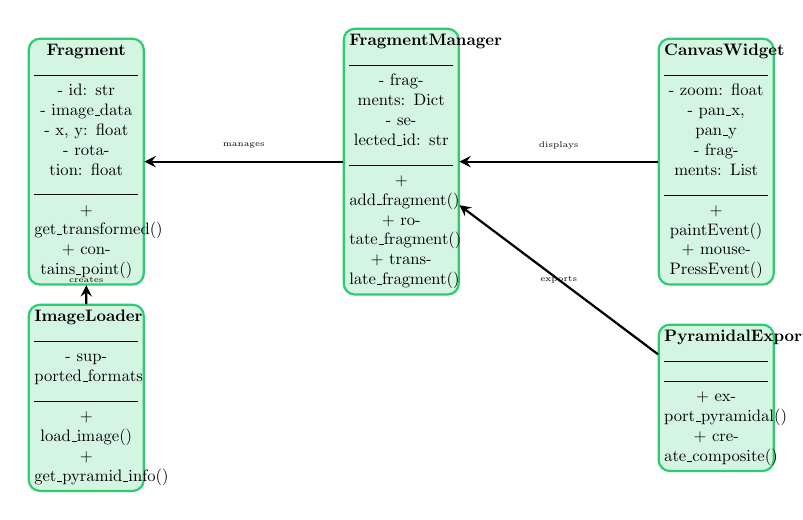
\begin{tikzpicture}[node distance=2cm, every node/.style={scale=0.6}]

% Classes principales
\node (fragment) [process, text width=2.2cm] at (0,3) {
    \textbf{Fragment}\\
    \rule{2.2cm}{0.4pt}\\
    - id: str\\
    - image\_data\\
    - x, y: float\\
    - rotation: float\\
    \rule{2.2cm}{0.4pt}\\
    + get\_transformed()\\
    + contains\_point()
};

\node (fragmgr) [process, text width=2.2cm] at (4,3) {
    \textbf{FragmentManager}\\
    \rule{2.2cm}{0.4pt}\\
    - fragments: Dict\\
    - selected\_id: str\\
    \rule{2.2cm}{0.4pt}\\
    + add\_fragment()\\
    + rotate\_fragment()\\
    + translate\_fragment()
};

\node (canvas) [process, text width=2.2cm] at (8,3) {
    \textbf{CanvasWidget}\\
    \rule{2.2cm}{0.4pt}\\
    - zoom: float\\
    - pan\_x, pan\_y\\
    - fragments: List\\
    \rule{2.2cm}{0.4pt}\\
    + paintEvent()\\
    + mousePressEvent()
};

\node (loader) [process, text width=2.2cm] at (0,0) {
    \textbf{ImageLoader}\\
    \rule{2.2cm}{0.4pt}\\
    - supported\_formats\\
    \rule{2.2cm}{0.4pt}\\
    + load\_image()\\
    + get\_pyramid\_info()
};

\node (exporter) [process, text width=2.2cm] at (8,0) {
    \textbf{PyramidalExporter}\\
    \rule{2.2cm}{0.4pt}\\
    \rule{2.2cm}{0.4pt}\\
    + export\_pyramidal()\\
    + create\_composite()
};

% Relations
\draw [arrow] (fragmgr) -- (fragment);
\draw [arrow] (canvas) -- (fragmgr);
\draw [arrow] (loader) -- (fragment);
\draw [arrow] (exporter) -- (fragmgr);

% Labels des relations
\node at (2,3.2) {\tiny manages};
\node at (6,3.2) {\tiny displays};
\node at (0,1.5) {\tiny creates};
\node at (6,1.5) {\tiny exports};

\end{tikzpicture}
\caption{Diagramme de classes simplifié}
\label{fig:diagramme_classes}
\end{figure}

\subsection{Flux d'exécution détaillé}

Le flux d'exécution de l'application suit un modèle événementiel basé sur le système de signaux/slots de Qt :

\textbf{Phase de prétraitement} :
\begin{enumerate}
\item Utilisation de QuPath pour la lecture des images numériques (formats SVS, MRXS)
\item Exploitation du plugin Segment Anything Model (SAM) pour délimiter les zones de tissu
\item Export du masque correspondant au format GeoJSON
\item Exécution du pipeline unifié prenant en entrée l'image originale et le fichier GeoJSON
\item Génération d'un fichier TIFF pyramidal contenant uniquement le tissu extrait au format RGBA
\end{enumerate}

\textbf{Phase de suture} :
\begin{enumerate}
\item Import des fragments obtenus dans l'outil desktop
\item Alignement et assemblage manuel des fragments par l'utilisateur
\item Export des fragments suturés au format TIFF pyramidal avec sélection du niveau de détail
\end{enumerate}

\section{Analyse critique et perspectives}

\subsection{Points forts de la solution}

\textbf{Adaptation aux besoins spécifiques} : La solution développée répond précisément aux besoins identifiés lors de l'analyse du cahier des charges, sans fonctionnalités superflues qui pourraient complexifier l'utilisation.

\textbf{Performance optimisée} : L'architecture développée permet de traiter efficacement des images de très haute résolution tout en maintenant une interface réactive. Les optimisations implémentées (cache multi-niveaux, rendu adaptatif, gestion mémoire) garantissent des performances satisfaisantes même sur des configurations matérielles standard.

\textbf{Extensibilité} : L'architecture modulaire facilite l'ajout de nouvelles fonctionnalités et l'adaptation à de nouveaux besoins. Le pattern MVC et l'utilisation de signaux/slots permettent une évolution incrémentale sans refactoring majeur.

\textbf{Robustesse} : Les tests approfondis et la validation utilisateur garantissent la fiabilité de la solution en conditions réelles. La gestion d'erreurs complète et les mécanismes de récupération assurent une expérience utilisateur stable.

\subsection{Limitations identifiées}

\textbf{Dépendance aux bibliothèques natives} : L'utilisation de bibliothèques C/C++ (OpenSlide, VIPS) complexifie le déploiement et la maintenance. Une évolution vers des solutions plus portables pourrait améliorer l'adoption.

\textbf{Alignement manuel} : L'absence d'algorithmes d'alignement automatique robustes limite l'efficacité pour certains types de fragments. L'intégration d'assistance automatique pourrait accélérer le processus.

\textbf{Formats supportés} : La solution se concentre actuellement sur les formats SVS et MRXS, mais l'écosystème comprend d'autres formats propriétaires.

\subsection{Perspectives d'évolution}

\textbf{Intelligence artificielle} : L'intégration d'algorithmes d'apprentissage automatique pourrait améliorer la segmentation automatique et l'alignement des fragments. Les modèles de vision transformer récents offrent des perspectives prometteuses.

\textbf{Collaboration temps réel} : Le développement de fonctionnalités collaboratives permettrait à plusieurs utilisateurs de travailler simultanément sur la même reconstitution.

\textbf{Intégration workflow} : Une meilleure intégration avec les systèmes d'information hospitaliers faciliterait l'adoption en routine clinique.

\textbf{Analyse quantitative} : L'ajout de fonctionnalités d'analyse quantitative transformerait l'outil en plateforme d'analyse complète.

\chapter{Développement Durable et Responsabilité Sociétale}

\section{Impact environnemental}

Le développement de cet outil s'inscrit dans une démarche de responsabilité environnementale à plusieurs niveaux. Premièrement, la numérisation et le traitement informatique des lames histologiques contribuent à réduire l'utilisation de ressources physiques traditionnellement nécessaires à l'analyse anatomopathologique. En permettant une manipulation entièrement numérique des échantillons, l'outil réduit le besoin de manipulations physiques répétées des lames, limitant ainsi les risques de dégradation et la nécessité de nouvelles préparations.

L'optimisation des performances de l'application contribue également à réduire l'empreinte énergétique. Les algorithmes de mise en cache et de gestion des niveaux de détail minimisent l'utilisation des ressources computationnelles, réduisant ainsi la consommation électrique des postes de travail. Cette approche s'aligne avec les objectifs de sobriété numérique promus dans le secteur de la santé.

\section{Bénéfices sociétaux}

L'outil développé présente des bénéfices sociétaux significatifs dans le domaine de la santé publique. En améliorant la précision et l'efficacité de l'analyse anatomopathologique, il contribue indirectement à l'amélioration des diagnostics médicaux et, par conséquent, à la qualité des soins prodigués aux patients.

La réduction du temps nécessaire à la reconstitution des lames fragmentées permet aux anatomopathologistes de consacrer plus de temps à l'analyse diagnostique proprement dite, améliorant ainsi la productivité du système de santé. Cette efficacité accrue est particulièrement importante dans un contexte de pénurie de spécialistes en anatomopathologie.

L'outil favorise également la démocratisation de l'accès à des technologies avancées d'imagerie médicale. En développant une solution open-source et facilement déployable, le projet contribue à réduire les inégalités d'accès aux outils diagnostiques de pointe entre différents établissements de santé.

\section{Considérations éthiques}

Le développement de l'outil a intégré des considérations éthiques importantes liées à la manipulation de données médicales sensibles. L'architecture de l'application privilégie le traitement local des données, évitant ainsi les risques liés au transfert et au stockage de données patient sur des serveurs distants.

La transparence des algorithmes utilisés constitue un autre aspect éthique important. Contrairement aux solutions basées sur l'intelligence artificielle "boîte noire", l'outil développé utilise des transformations géométriques explicites et vérifiables, permettant aux utilisateurs de comprendre et de valider chaque étape du processus de reconstitution.

\chapter{Conclusion}

\section{Bilan du stage}

Ce stage de spécialité au Centre Henri Becquerel a constitué une expérience particulièrement enrichissante, tant sur le plan technique que professionnel. Le développement d'un outil de génération d'images d'anatomopathologie de haute définition m'a permis d'appliquer concrètement les connaissances acquises durant ma formation d'ingénieur tout en découvrant les spécificités du domaine médical.

L'approche méthodologique adoptée, combinant analyse des besoins, étude comparative des solutions existantes, et développement itératif, illustre parfaitement la démarche ingénieur. Cette expérience a renforcé ma compréhension de l'importance de l'analyse préalable et de la validation continue avec les utilisateurs finaux dans le développement de solutions techniques.

Sur le plan technique, ce projet m'a permis d'approfondir mes compétences en traitement d'images, développement d'interfaces graphiques, et optimisation des performances. La gestion d'images de très haute résolution et les contraintes de performance en temps réel ont constitué des défis techniques stimulants qui ont enrichi mon expertise.

L'environnement pluridisciplinaire du Centre Henri Becquerel a également été formateur, me permettant de collaborer avec des médecins, physiciens médicaux, et chercheurs. Cette expérience a développé mes capacités de communication technique et ma compréhension des enjeux spécifiques au domaine médical.

\section{Apports personnels et professionnels}

Ce stage a considérablement enrichi mon profil professionnel en me permettant d'acquérir une expertise dans un domaine d'application spécialisé et en forte croissance : l'imagerie médicale numérique. Les compétences développées en traitement d'images haute résolution, optimisation des performances, et développement d'interfaces utilisateur spécialisées constituent des atouts précieux pour ma future carrière.

L'expérience de développement d'une solution complète, depuis l'analyse des besoins jusqu'au déploiement, m'a permis de développer une vision globale du cycle de développement logiciel. Cette approche holistique est essentielle pour un ingénieur et complète parfaitement la formation théorique reçue à l'INSA.

La collaboration avec des utilisateurs finaux experts dans leur domaine a également développé mes capacités d'écoute, d'analyse des besoins, et d'adaptation des solutions techniques aux contraintes métier. Ces compétences transversales sont essentielles dans le contexte professionnel actuel.

\section{Perspectives d'évolution}

Plusieurs axes d'évolution prometteurs ont été identifiés pour améliorer et étendre les capacités de l'outil.

\textbf{Intelligence artificielle} : L'intégration d'algorithmes d'apprentissage automatique pourrait considérablement améliorer l'efficacité de la segmentation et de l'alignement. Les récents progrès en vision par ordinateur, notamment les modèles de type Vision Transformer, offrent des perspectives intéressantes pour l'analyse automatique des structures histologiques.

\textbf{Collaboration en temps réel} : Le développement de fonctionnalités collaboratives permettrait à plusieurs anatomopathologistes de travailler simultanément sur la même reconstitution, facilitant les consultations pluridisciplinaires et l'enseignement.

\textbf{Intégration workflow} : Une meilleure intégration avec les systèmes d'information hospitaliers (SIH) et les systèmes de gestion des laboratoires (LIMS) faciliterait l'adoption en routine clinique et améliorerait la traçabilité des analyses.

En conclusion, ce stage a permis de développer une solution technique répondant à un besoin concret tout en contribuant à l'avancement des pratiques en anatomopathologie numérique. Les résultats obtenus et les perspectives d'évolution identifiées confirment la pertinence de l'approche adoptée et ouvrent la voie à de futurs développements dans ce domaine en pleine expansion.

\begin{thebibliography}{20}

\bibitem{openslide}
Goode, A., Gilbert, B., Harkes, J., Jukic, D., \& Satyanarayanan, M. (2013). 
\textit{OpenSlide: A vendor-neutral software foundation for digital pathology}. 
Journal of Pathology Informatics, 4(1), 27.

\bibitem{qupath}
Bankhead, P., Loughrey, M. B., Fernández, J. A., Dombrowski, Y., McArt, D. G., Dunne, P. D., ... \& Hamilton, P. W. (2017). 
\textit{QuPath: Open source software for digital pathology image analysis}. 
Scientific Reports, 7(1), 16878.

\bibitem{sam}
Kirillov, A., Mintun, E., Ravi, N., Mao, H., Rolland, C., Gustafson, L., ... \& Girshick, R. (2023). 
\textit{Segment anything}. 
arXiv preprint arXiv:2304.02643.

\bibitem{vips}
Martinez, K., \& Cupitt, J. (2005). 
\textit{VIPS–a highly tuned image processing software architecture}. 
In IEEE International Conference on Image Processing 2005 (Vol. 2, pp. II-574).

\bibitem{pyqt}
Summerfield, M. (2015). 
\textit{Rapid GUI programming with Python and Qt: the definitive guide to PyQt programming}. 
Prentice Hall Professional.

\bibitem{tiff}
Adobe Systems Incorporated. (1992). 
\textit{TIFF Revision 6.0 Final Specification}. 
Adobe Systems Incorporated.

\bibitem{sift}
Lowe, D. G. (2004). 
\textit{Distinctive image features from scale-invariant keypoints}. 
International Journal of Computer Vision, 60(2), 91-110.

\bibitem{digital_pathology}
Pantanowitz, L., Valenstein, P. N., Evans, A. J., Kaplan, K. J., Pfeifer, J. D., Wilbur, D. C., ... \& Colgan, T. J. (2011). 
\textit{Review of the current state of whole slide imaging in pathology}. 
Journal of Pathology Informatics, 2(1), 36.

\bibitem{image_stitching}
Brown, M., \& Lowe, D. G. (2007). 
\textit{Automatic panoramic image stitching using invariant features}. 
International Journal of Computer Vision, 74(1), 59-73.

\bibitem{medical_imaging}
Doi, K. (2007). 
\textit{Computer-aided diagnosis in medical imaging: historical review, current status and future potential}. 
Computerized Medical Imaging and Graphics, 31(4-5), 198-211.

\bibitem{histopathology}
Kumar, N., Verma, R., Sharma, S., Bhargava, S., Vahadane, A., \& Sethi, A. (2017). 
\textit{A dataset and a technique for generalized nuclear segmentation for computational pathology}. 
IEEE Transactions on Medical Imaging, 36(7), 1550-1560.

\bibitem{performance_optimization}
Fog, A. (2020). 
\textit{Optimizing software in C++: An optimization guide for Windows, Linux and Mac platforms}. 
Copenhagen University College of Engineering.

\bibitem{tepmargins}
Centre Henri Becquerel. (2024). 
\textit{Protocole TEP Margins : Évaluation des marges chirurgicales par micro-TEP TDM}. 
Documentation interne, Département d'Imagerie Médicale.

\bibitem{anatomopathologie}
Rosai, J. (2011). 
\textit{Rosai and Ackerman's Surgical Pathology}. 
10th Edition, Elsevier.

\bibitem{pyramidal_imaging}
Herrmann, M. D., Clunie, D. A., Fedorov, A., Doyle, S. W., Pieper, S., Klepeis, V., ... \& Kikinis, R. (2018). 
\textit{Implementing the DICOM standard for digital pathology}. 
Journal of Pathology Informatics, 9(1), 37.

\end{thebibliography}

\end{document}